\section{VIX futures: head-to-head \RoughCert{} audit of published benchmarks}\label{sec:vix_futures}

Under the rough Bergomi model \citep{BayerFrizGatheral2016}, the squared VIX index at maturity $T$ over
the forward window $\Delta$ is the Wick-exponential functional \eqref{eq:vix2_def}. Different articles
use two distinct kernel normalisations and window lengths:
\begin{itemize}
\item \citet{BayerFrizGatheral2016}, \citet{JacquierMartiniMuguruza2018}, and \citet{BonesiniCallegaroJacquier2023}
  write $K(u,s)=\eta_{\mathrm{P1}}\sqrt{2H}(u-s)^{H-1/2}$ (with $\Delta=30/365$ or $\Delta=1/12$);
\item \citet{BourgeyDeMarco2022} and \citet{BourgeyDeMarcoGobet2023} write $K(u,s)=a(u-s)^{H-1/2}$ with
  $\Delta=1/12$, where $a=\eta_{\mathrm{P1}}\sqrt{2H}$.
\end{itemize}
Every table below states $(H,T,\Delta,a)$ explicitly so no comparison mixes conventions. All VIX futures
prices are quoted in volatility points ($100\times\mathrm{VIX}_T$), where one standard Cboe futures tick
equals $0.05$ volatility points \citep{CBOE2024VIX}. Every enclosure in this section is \lab{Arb-certified}.

\subsection{Headline \RoughCertTilt{} audit: separating published expansions by more than one tick}\label{sec:vix_headline}
Table~\ref{tab:vix_headline} summarises our 169-bit Arb \RoughCertTilt{} verification across eight headline parameter cells
covering literature configurations and E14 base and stress tests. Every cell passes our strict outward-rounded enclosure
gate (total bracket width below $0.05$ points and Arb endpoint enclosure width at most $1.39\times10^{-3}$ points
for $L$ and $6.41\times10^{-11}$ points for $U$). Three decisive findings emerge directly from the
outward-rounded intervals:
\begin{enumerate}
\item \emph{Machine-verified $>1$ tick violation by BDG~(2023) in stress regimes.} In the six-month
  stress cell ($H=0.10$, $T=0.5$, $\eta_{\mathrm{P1}}=3.0$, $a=1.34164$, $\Delta=30/365$), the static
  \RoughCertTilt{} bracket is $[\ArbStressTiltedL,\ArbStressTiltedU]$ (width $\ArbStressTiltedW$ points), while
  our independent Arb evaluation of \citet[Theorem~2.2]{BourgeyDeMarcoGobet2023} gives $\ArbStressBDG$
  points---exceeding the continuous rough-Bergomi upper bound $U$ by at least $+\ArbStressBDGGap$ points
  ($\TickStress$ Cboe ticks; and by $+\GapStressRefined$ points, or $\TickStressRefined$ ticks, using the refined \RoughCertCV{} upper bound
  of Section~\ref{sec:vix_options}). On BDG's own Figure~1 extreme cell ($H=0.10$, $T=0.5$,
  $a=1.5$, $\Delta=1/12$), the \RoughCertTilt{} bracket is $[\ArbFigOneL,\ArbFigOneU]$ (width $\ArbFigOneW$
  points) while BDG~(2023) gives $\ArbFigOneBDG$, certifying an upward bias of at least
  $+\ArbFigOneBDGGap$ points ($\TickFigOne$ Cboe ticks). Even at ultra-rough $H=0.05$ ($\eta_{\mathrm{P1}}=3.0$,
  $T=0.5$, Table~\ref{tab:vix_e14}), the observed BDG excess reaches $+\ArbStressHZeroFiveBDGGap$ points
  ($\TickStressHZeroFive$ ticks).
\item \emph{Certified downward bias of the moment-matched lognormal proxy.} Across all eight headline
  cells, the exact moment-matched lognormal proxy $F_{\mathrm{LN}}=M_1^{3/4}M_2^{-1/8}$ lies strictly
  below our Arb lower bound $L$. Its downward bias exceeds one Cboe tick not only in stress
  ($-\ArbStressLNGap$ points in E14 stress and $-\ArbFigOneLNGap$ points at $a=1.5$, or $\TickLNStress$--$\TickLNFigOne$
  ticks), but already in moderate regimes: $-\LNGapFigSix$ points ($\TickLNFigSix$ ticks) in BDG Figure~6 ($a=1.0$,
  $T=3$\,m) and $-\LNGapBCJ$ points ($\TickLNBCJ$ ticks) in BCJ~\S5.3 ($H=0.10$, $\eta_{\mathrm{P1}}=1.9$,
  $T=6$\,m).
\item \emph{Disentangling continuum and $500$-cell grid targets in Bourgey and De Marco~(2022).}
  On the multilevel Monte Carlo benchmark of \citet[Section~3.3]{BourgeyDeMarco2022} ($H=0.10$, $T=0.5$,
  $a=0.5$, $\Delta=1/12$, published MLMC price $22.18135$), the continuous-time Arb bracket is
  $[\ArbBDContL,\ArbBDContU]$ (width $\ArbBDContW$ points), whereas the exact Arb tilted bracket for
  their $500$-cell right-rectangle discrete target $\Lambda_{500}=\frac{1}{500}\sum_{j=1}^{500}\xi_T(T+j\Delta/500)$
  (zero spatial discretisation error) is $[\ArbBDGridL,\ArbBDGridU]$ (Figure~\ref{fig:vix_bcj_disjoint}(a)).
  The two Arb intervals are strictly disjoint by at least $\ArbBDDisjointGap$ points, and the published
  MLMC value $22.18135$ sits strictly inside the $500$-cell Arb enclosure, at least $\MLMCBelowGridU$ points
  below its upper endpoint. The reported estimate is compatible with its declared grid and falls outside the continuum interval.
\end{enumerate}

\IfFileExists{tables/tab_vix_headline.tex}{\begin{table}[!htbp]\centering\scriptsize\setlength{\tabcolsep}{2.2pt}
\caption{Headline 169-bit Arb-certified \RoughCertTilt{} VIX futures brackets (volatility points) across eight literature and stress-test parameter cells, audited against BDG~(2023) and lognormal proxies.}\label{tab:vix_headline}
\begin{tabular}{@{}lrrrrccrrr@{}}\toprule
 & \multicolumn{4}{c}{Contract parameters} & \multicolumn{2}{c}{\textbf{\RoughCertTilt{}} (pts)} & \multicolumn{3}{c}{Expansion and signed gaps (pts)} \\
\cmidrule(lr){2-5}\cmidrule(lr){6-7}\cmidrule(lr){8-10}
Benchmark & $H$ & $T$ (yr) & $\Delta$ (yr) & $a$ & $[L,\,U]$ & Width & BDG$_3$ & $\mathrm{BDG}_3\!-\!U$ & $\mathrm{LN}\!-\!L$ \\\midrule
Stress (E14) & 0.10 & 0.50 & 30/365 & 1.342 & \textbf{\boldmath [15.53706,\,15.55718]} & \textbf{\boldmath 0.02011} & 15.61414 & $+$0.05696$^\star$ & $-$0.2965$^\star$ \\
BDG (2023) Fig.~1 & 0.10 & 0.50 & 1/12 & 1.500 & \textbf{\boldmath [14.05216,\,14.08195]} & \textbf{\boldmath 0.02978} & 14.16307 & $+$0.08112$^\star$ & $-$0.4304$^\star$ \\
BD (2022) \S3.3 & 0.10 & 0.50 & 1/12 & 0.500 & \textbf{\boldmath [22.17993,\,22.18038]} & \textbf{\boldmath 0.00044} & 22.18192 & $+$0.00154 & $-$0.0076 \\
BDG (2023) Fig.~6 & 0.10 & 0.25 & 1/12 & 1.000 & \textbf{\boldmath [19.90857,\,19.91515]} & \textbf{\boldmath 0.00657} & 19.93666 & $+$0.02152 & $-$0.0978$^\star$ \\
BCJ (2023) \S5.3 & 0.10 & 0.50 & 1/12 & 0.850 & \textbf{\boldmath [19.81201,\,19.81546]} & \textbf{\boldmath 0.00345} & 19.82707 & $+$0.01161 & $-$0.0581$^\star$ \\
Base ($H=0.10$) & 0.10 & 1/12 & 30/365 & 0.850 & \textbf{\boldmath [22.01885,\,22.02193]} & \textbf{\boldmath 0.00307} & 22.03265 & $+$0.01073 & $-$0.0358 \\
Base ($H=0.05$) & 0.05 & 1/12 & 30/365 & 0.601 & \textbf{\boldmath [22.50390,\,22.50644]} & \textbf{\boldmath 0.00254} & 22.51588 & $+$0.00943 & $-$0.0214 \\
Stress ($H=0.30$) & 0.30 & 0.50 & 30/365 & 2.324 & \textbf{\boldmath [12.66828,\,12.66937]} & \textbf{\boldmath 0.00108} & 12.67214 & $+$0.00278 & $-$0.0680$^\star$ \\
\midrule
BD (2022) 500-cell & 0.10 & 0.50 & 1/12 & 0.500 & \textbf{\boldmath [22.18102,\,22.18141]} & \textbf{\boldmath 0.00039} & \multicolumn{3}{c}{MLMC $= 22.18135$ (inside grid band)} \\
\bottomrule\end{tabular}
\smallskip\par\raggedright\scriptsize\emph{Notes:} Bold identifies the tilted interval and width before display rounding. $H$ is the Hurst exponent, $T$ maturity, $\Delta$ the window and $a=\eta_{\mathrm{P1}}\sqrt{2H}$. BDG$_3$ is the third-order expansion; LN is lognormal. Signed gaps use the nearest bound. $^\star$ exceeds one Cboe tick ($0.05$ pts). Endpoint enclosure widths (at most $1.4\times 10^{-3}$ pts) are included.
\end{table}
}{}

\subsection{Complete 15-cell E14 suite and JMM~(2018) lower-bound audit}\label{sec:vix_e14}
Table~\ref{tab:vix_e14} extends the audit to all $15$ cells of the base, curved-$\xi_0$
\citep[Scenario~2: $\xi_0(t)=0.234^2(1+t)^2$]{JacquierMartiniMuguruza2018}, and stress design
($\Delta=30/365$), taking the sharpest outward-rounded Arb bracket from Theorem~\ref{thm:tilted} and
Proposition~\ref{prop:arb}. Every cell resolves well below one Cboe tick: maximum width is
$\ArbEFourteenBaseMaxW$ points across the $12$ base and curved cells and $\ArbEFourteenMaxW$ points across
all $15$ cells, narrowing the published bounds of \citet[Theorem~3.3]{JacquierMartiniMuguruza2018} by
factors of $\ArbJMMRatioLo\times$ to $\ArbJMMRatioHi\times$. To credit the strength of JMM~(2018) fairly,
Table~\ref{tab:vix_e14} also reports $U-L_{\mathrm{JMM}}$, the worst-case error of JMM's lower bound
alone: JMM's lower bound is accurate to within $0.008$--$0.105$ points in base and curved cells (reaching
$0.146$--$0.152$ points for the $H=0.05,0.10$ stress cells), while the massive width ratio reflects JMM's variance-swap
upper bound $\sqrt{\E[\mathrm{VIX}_T^2]}$. Our Arb bounds sharpen both sides simultaneously without a
reference simulation, with timings reported separately in the archive.

\IfFileExists{tables/tab_vix_e14_15cells.tex}{\begin{table}[!htbp]\centering\scriptsize\setlength{\tabcolsep}{3.6pt}
\caption{Complete 15-cell Arb-certified \RoughCert{} VIX futures suite (volatility points, $\Delta=30/365$), benchmarked against JMM~(2018), BDG~(2023), and lognormal proxies.}\label{tab:vix_e14}
\begin{tabular}{@{}rlcrrrrrr@{}}\toprule
 & & \multicolumn{2}{c}{\textbf{\RoughCert{}} (pts)} & \multicolumn{3}{c}{JMM (2018) bounds} & \multicolumn{2}{c}{Certified proxy gap (pts)} \\
\cmidrule(lr){3-4}\cmidrule(lr){5-7}\cmidrule(lr){8-9}
$H$ & $T$ & $[L,\,U]$ & Width & \shortstack{Width\\(pts)} & \shortstack{Lower-bound\\error limit (pts)} & \shortstack{Width\\ratio} & $\mathrm{BDG}_3-U$ & $\mathrm{LN}-L$ \\\midrule
\multicolumn{9}{@{}l}{\emph{Panel A: Base regime ($\eta_{\mathrm{P1}}=1.9$, flat $\xi_0=0.235^2$)}} \\
\addlinespace[1.5pt]
0.05 & 1w & \textbf{\boldmath [23.12106,\,23.12218]} & \textbf{\boldmath 0.00111} & 0.427 & 0.0491 & 385$\times$ & $+$0.00667 & $-$0.0078 \\
0.05 & 1m & \textbf{\boldmath [22.50405,\,22.50644]} & \textbf{\boldmath 0.00238} & 1.056 & 0.0622 & 443$\times$ & $+$0.00943 & $-$0.0216 \\
0.05 & 3m & \textbf{\boldmath [21.77897,\,21.78174]} & \textbf{\boldmath 0.00277} & 1.783 & 0.0641 & 645$\times$ & $+$0.01015 & $-$0.0306 \\
0.10 & 1w & \textbf{\boldmath [22.96234,\,22.96354]} & \textbf{\boldmath 0.00119} & 0.589 & 0.0516 & 494$\times$ & $+$0.00708 & $-$0.0121 \\
0.10 & 1m & \textbf{\boldmath [22.01917,\,22.02193]} & \textbf{\boldmath 0.00275} & 1.546 & 0.0675 & 563$\times$ & $+$0.01073 & $-$0.0361 \\
0.10 & 3m & \textbf{\boldmath [20.83240,\,20.83583]} & \textbf{\boldmath 0.00343} & 2.734 & 0.0698 & 799$\times$ & $+$0.01165 & $-$0.0525$^\star$ \\
0.30 & 1w & \textbf{\boldmath [23.06690,\,23.06697]} & \textbf{\boldmath 0.00006} & 0.442 & 0.0084 & 7,679$\times$ & $+$0.00022 & $-$0.0016 \\
0.30 & 1m & \textbf{\boldmath [22.01988,\,22.02002]} & \textbf{\boldmath 0.00014} & 1.493 & 0.0126 & 11,449$\times$ & $+$0.00048 & $-$0.0070 \\
0.30 & 3m & \textbf{\boldmath [20.20115,\,20.20133]} & \textbf{\boldmath 0.00017} & 3.313 & 0.0138 & 19,586$\times$ & $+$0.00060 & $-$0.0129 \\
\midrule
\multicolumn{9}{@{}l}{\emph{Panel B: Curved forward variance ($\eta_{\mathrm{P1}}=1.9$, JMM Scenario~2: $\xi_0(t)=0.234^2(1+t)^2$)}} \\
\addlinespace[1.5pt]
0.05 & 1m & \textbf{\boldmath [25.21964,\,25.22259]} & \textbf{\boldmath 0.00294} & 1.190 & 0.0948 & 405$\times$ & --- & --- \\
0.10 & 1m & \textbf{\boldmath [24.68133,\,24.68480]} & \textbf{\boldmath 0.00346} & 1.737 & 0.1042 & 502$\times$ & --- & --- \\
0.30 & 1m & \textbf{\boldmath [24.66989,\,24.67087]} & \textbf{\boldmath 0.00098} & 1.682 & 0.0346 & 1,731$\times$ & --- & --- \\
\midrule
\multicolumn{9}{@{}l}{\emph{Panel C: Stress regime ($\eta_{\mathrm{P1}}=3.0$, $T=6$\,m, flat $\xi_0=0.235^2$)}} \\
\addlinespace[1.5pt]
0.05 & 6m & \textbf{\boldmath [18.26959,\,18.28359]} & \textbf{\boldmath 0.01399} & 5.363 & 0.1463 & 383$\times$ & $+$0.05525$^\star$ & $-$0.1920$^\star$ \\
0.10 & 6m & \textbf{\boldmath [15.54052,\,15.55650]} & \textbf{\boldmath 0.01598} & 8.096 & 0.1516 & 506$\times$ & $+$0.05764$^\star$ & $-$0.3000$^\star$ \\
0.30 & 6m & \textbf{\boldmath [12.66836,\,12.66937]} & \textbf{\boldmath 0.00101} & 10.860 & 0.0293 & 10,852$\times$ & $+$0.00278 & $-$0.0680$^\star$ \\
\bottomrule\end{tabular}
\smallskip\par\raggedright\scriptsize\emph{Notes:} Bold identifies the narrowest available \RoughCert{} interval and its width. $H$ is the Hurst exponent and $T$ maturity. The JMM error limit is $U-L_{\rm JMM}$; the ratio divides JMM width by \RoughCert{} width. BDG$_3$ is the third-order expansion; LN is lognormal. $^\star$ exceeds one Cboe tick ($0.05$ pts). A dash marks an unevaluated proxy.
\end{table}
}{}

\subsection{Parameter-space phase boundaries (BDG Figs.~1--2) and BCJ~(2023) multi-curve term structures}\label{sec:vix_sweeps}
Figure~\ref{fig:vix_phase_boundary} shows certified separations at the sampled parameters of BDG~(2023) and
the lognormal proxy across the two flagship parameter sweeps of \citet[Figures~1--2]{BourgeyDeMarcoGobet2023}
($T=0.5$, $\Delta=1/12$, $\xi_0=0.235^2$). Along the vol-of-vol sweep at $H=0.10$
(Figure~\ref{fig:vix_phase_boundary}(a)), the Arb tilted width, the observed BDG excess
$\mathrm{BDG}_3-U$, and the lognormal shortfall $L-\mathrm{LN}$ grow with $a$ (the width law is given by
Theorem~\ref{thm:tilted}(iii)), staying strictly ordered: the lognormal shortfall first exceeds the $0.05$-point Cboe tick on the sampled grid at $a=1.00$, following a sub-tick shortfall at $a=0.80$, whereas the lower bound on BDG's error lies below one tick at $a\approx1.20$ ($\mathrm{BDG}_3-U=\SweepAOneTwo$) and enters the Arb-certified $>1$-tick
violation zone at the sampled values $a=1.35,1.50$ ($+\SweepAOneThreeFive$ at $a=1.35$, $+\SweepAOneFive$ at $a=1.50$). Along the roughness sweep at $a=1.0$ (Figure~\ref{fig:vix_phase_boundary}(b)), decreasing $H$ from $0.40$
to $0.05$ amplifies both kernel dispersion and competitor biases sharply: at $H=0.05$ ($a=1.0$, $T=6$\,m),
even this moderate vol-of-vol drives BDG~(2023) above our Arb upper bound by at least $\SweepHBDG$ points
($\SweepHBDGTicks$ ticks) and the lognormal proxy below our Arb lower bound by at least $\SweepHLN$ points
($\SweepHLNTicks$ ticks), while our Arb width stays below $\SweepHWidth$ points (marginally above half a tick
at $H=0.05$, and below $\SweepHWidthRest$ points for $H\ge0.10$).

\begin{figure}[!htbp]\centering
\IfFileExists{figures/fig_v3_02_phase_boundaries.pdf}{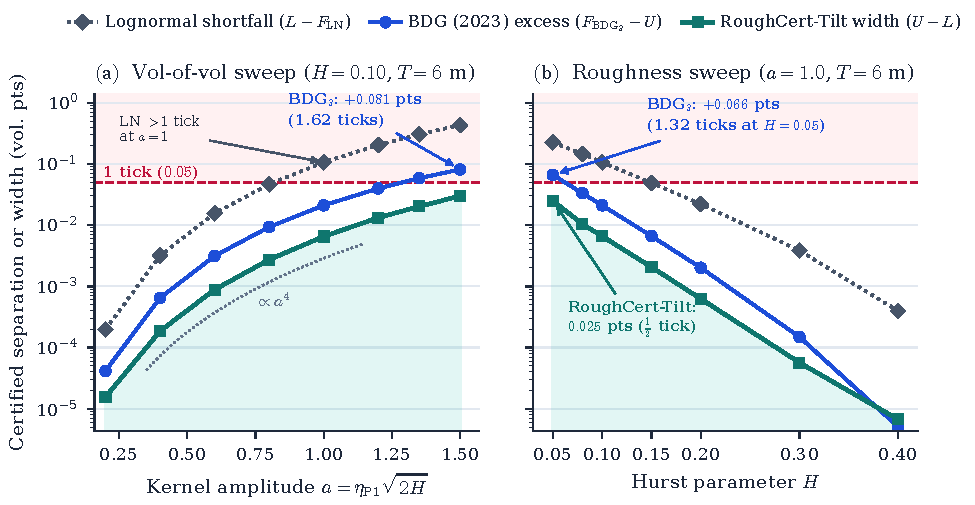
\includegraphics[width=\textwidth]{figures/fig_v3_02_phase_boundaries.pdf}}{\fbox{fig\_v3\_02 pending}}
\caption{Arb-certified bias of BDG~(2023) ($F_{\mathrm{BDG}_3}-U$) and lognormal proxy ($L-F_{\mathrm{LN}}$)
versus \RoughCertTilt{} width ($U-L$) at $T=6$\,m. (a) Vol-of-vol $a$ sweep ($H=0.10$); (b) Hurst $H$ sweep
($a=1.0$). Shaded region exceeds one Cboe tick ($0.05$ pts).}\label{fig:vix_phase_boundary}
\end{figure}

To benchmark against the functional quantisation suite of \citet[Section~5.3]{BonesiniCallegaroJacquier2023}
($H=0.10$, $\eta_{\mathrm{P1}}=1.9$, $\Delta=1/12$), we evaluate all $18$ combinations of their three
forward-variance curves ($\xi_0(t)=0.234^2\{1,(1+t)^2,\sqrt{1+t}\}$) and six maturities
($T\in\{1,2,3,6,9,12\}$ months; Figure~\ref{fig:vix_bcj_disjoint}(b) and Supplementary Table~S1).
Because the unweighted barycentre $h_0$ keeps the exact Pfaff ${}_2F_1$ inner products across arbitrary
curves, \RoughCertCV{} (Proposition~\ref{prop:arb}(c)--(d)) certifies every continuous-time future to width
at most $\ArbBCJMaxW$ points ($\ArbBCJRatioLo\times$--$\ArbBCJRatioHi\times$ narrower than JMM~2018),
while the 960-path BCJ quantiser sits visibly below all three term structures.

\begin{figure}[!htbp]\centering
\IfFileExists{figures/fig_v3_03_disjoint_and_curves.pdf}{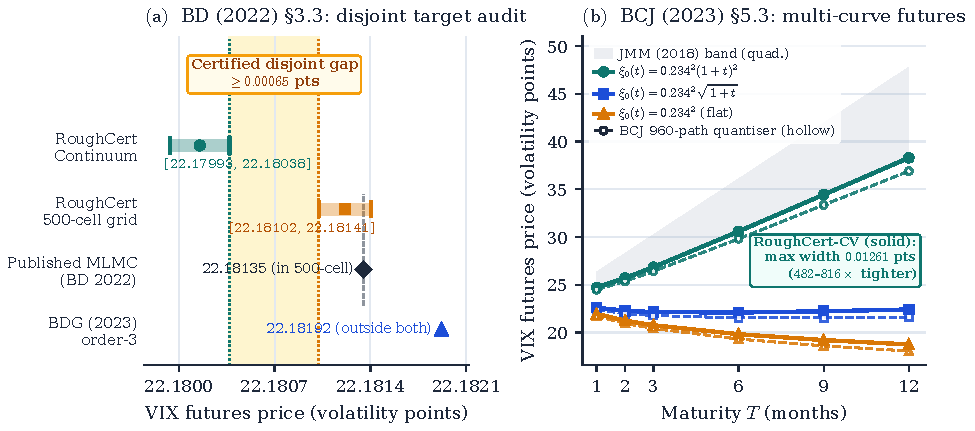
\includegraphics[width=\textwidth]{figures/fig_v3_03_disjoint_and_curves.pdf}}{\fbox{fig\_v3\_03 pending}}
\caption{(a) Disjoint 169-bit \RoughCertTilt{} enclosures for the continuum and $500$-cell grid in
\citet[Section~3.3]{BourgeyDeMarco2022}, isolating the published MLMC value ($22.18135$) inside the grid
target. (b) \RoughCertCV{} futures term structures versus BCJ~(2023) 960-path quantisers and JMM~(2018)
bounds.}\label{fig:vix_bcj_disjoint}
\end{figure}

\subsection{Extension to mixed rough Bergomi futures}\label{sec:mixed_rbergomi}
In mixed rough Bergomi the forward variance is a $\lambda$-weighted mixture of Wick exponentials with distinct
vol-of-vol levels, so no single exponential tilt reproduces its law. Conditioning on the shared Gaussian factor
$Z=W(h_0)/\norm{h_0}$ in Proposition~\ref{prop:arb}(c)--(d) instead retains the full nonlinear mixture inside
$X(z)$ while keeping the residual covariance $D_0$ tiny. Table~\ref{tab:vix_mixed} reports five mixed rough Bergomi cells ($H=0.10$, $\Delta=1/12$,
$\xi_0=0.235^2$): Scenario~1 $(a_1,a_2,\lambda)=(1.4,0.7,0.3)$ at $T\in\{1,3,6\}$ months and a higher
vol-of-vol stress mixture $(1.6,0.7,0.4)$ at $T\in\{3,6\}$ months. Across Scenario~1, the Arb brackets
achieve widths of at most $\ArbMixScenMaxW$ points ($<1/8$ of one Cboe tick), while BDG's order-three
mixed expansion, evaluated by floating-point quadrature, exceeds the respective upper endpoints by
approximately $+\MixScenGapLo$ to $+\MixScenGapHi$ points; under the stress mixture, the
observed BDG excess widens to $+\ArbMixMaxBDGGap$ points while our Arb width stays below
$\ArbMixAllMaxW$ points.

\IfFileExists{tables/tab_vix_mixed.tex}{\begin{table}[!htbp]\centering\footnotesize\setlength{\tabcolsep}{4.0pt}
\caption{Mixed rough Bergomi VIX futures (volatility points, $H=0.10$, $\Delta=1/12$, $\xi_0=0.235^2$): \RoughCertCV{} enclosures versus BDG~(2023) mixed weak expansions.}\label{tab:vix_mixed}
\begin{tabular}{@{}lcrccrrrr@{}}\toprule
 & & & \multicolumn{2}{c}{\textbf{\RoughCertCV{}} (pts)} & \multicolumn{3}{c}{BDG (2023) mixed (pts)} & \\
\cmidrule(lr){4-5}\cmidrule(lr){6-8}
Regime & $(a_1,a_2,\lambda)$ & $T$ & $[L,\,U]$ & Width & BDG$_0$ & BDG$_3$ & $\mathrm{BDG}_3-U$ & \shortstack{Setup / solve\\(s)} \\\midrule
Scenario~1 & (1.4,\,0.7,\,0.3) & 1m & \textbf{\boldmath [21.86821,\,21.87169]} & \textbf{\boldmath 0.00347} & 21.70815 & 21.88995 & $+$0.01826 & 1.8 / 5.2 \\
Scenario~1 & (1.4,\,0.7,\,0.3) & 3m & \textbf{\boldmath [20.63299,\,20.63780]} & \textbf{\boldmath 0.00481} & 20.47861 & 20.65502 & $+$0.01722 & 1.6 / 5.2 \\
Scenario~1 & (1.4,\,0.7,\,0.3) & 6m & \textbf{\boldmath [19.69027,\,19.69553]} & \textbf{\boldmath 0.00525} & 19.54665 & 19.71098 & $+$0.01546 & 1.5 / 5.0 \\
Stress & (1.6,\,0.7,\,0.4) & 3m & \textbf{\boldmath [19.85257,\,19.85950]} & \textbf{\boldmath 0.00692} & 19.65869 & 19.88916 & $+$0.02966 & 1.6 / 5.0 \\
Stress & (1.6,\,0.7,\,0.4) & 6m & \textbf{\boldmath [18.75046,\,18.75762]} & \textbf{\boldmath 0.00716} & 18.57762 & 18.78286 & $+$0.02523 & 1.4 / 4.8 \\
\bottomrule\end{tabular}
\smallskip\par\raggedright\scriptsize\emph{Notes:} Bold identifies the conditional-variance interval and width. $a_1,a_2$ are factor loadings, $\lambda$ is the mixing weight and $T$ is maturity in months. BDG$_0$ and BDG$_3$ denote zeroth- and third-order floating-point expansions. The signed gap compares the third-order value with the certified upper bound.
\end{table}
}{}
\ifTwoColumn\else\FloatBarrier\fi
